% This is samplepaper.tex, a sample chapter demonstrating the
% LLNCS macro package for Springer Computer Science proceedings;
% Version 2.20 of 2017/10/04
%
\documentclass[runningheads]{llncs}
%
\usepackage{graphicx}
\usepackage{float}
\usepackage{amsmath}
% Used for displaying a sample figure. If possible, figure files should
% be included in EPS format.
%
% If you use the hyperref package, please uncomment the following line
% to display URLs in blue roman font according to Springer's eBook style:
% \renewcommand\UrlFont{\color{blue}\rmfamily}

\begin{document}
%
\title{Automatic Concept Explanation for Deaf Users}
%
%\titlerunning{Abbreviated paper title}
% If the paper title is too long for the running head, you can set
% an abbreviated paper title here
%
\author{André Dias\inst{1} \and
Nuno Escudeiro\inst{2}}
%
\authorrunning{A. Dias, N. Escudeiro}
% First names are abbreviated in the running head.
% If there are more than two authors, 'et al.' is used.
%
\institute{Instituto Superior de Engenharia do Porto\\
\email{1140279@isep.ipp.pt}\and
Instituto Superior de Engenharia do Porto\\
\email{nfe@isep.ipp.pt}}
%
\maketitle              % typeset the header of the contribution
%
\begin{abstract}
    Concept explanation has a great importance in languages with small lexicons, such as sign languages.
    In Portugal, the official language used by the deaf community and the community that surrounds them is known as Língua Gestual Portuguesa (LGP).
    This language, like other sign languages has a small lexicon that is not able to represent all the words of the Portuguese language.
    The users of LGP, when faced with words like 'Nanotechnology' have to resort to tools made for Portuguese because the ones available to them are not ideal.
    Those solutions either lack a translation, which is the case of online dictionaries or aren't practical, which is the case of sign language interpreters.
    To solve this problem, this project was created with the hypothesis of verifying if it's possible to utilize Text Mining, Information Scraping and Information Retrieval techniques to generate the explanation of a given word or expression that does not exist in the LGP lexicon.
    The developed solution consists in an Application Programming Interface (API) capable of generating an explanation of a given word or expression.
    This API will feed a web application responsible for receiving the user input and presenting the explanation in plain text and its translation to LGP using an avatar.
    Although the development is not finished, the solution is already capable of displaying explanations in plain text that were generated with the mentioned techniques.

    \keywords{Sign language \and Text summarization \and Automatic concept explanation.}
\end{abstract}
%
%
%
\section{Introduction}

Concepts are abstract or generic ideas that have a common set of features that are shared across multiple situations and contexts.
Concept explanation can take a fundamental part of the learning process, whether it takes place in an educational environment, a day-to-day or a professional context.
The importance of concept explanation is even greater when it comes to languages with a small lexicon, in particular sign languages.

According to the World Health Organization \cite{who_2020}, as of march 2018, there were 466 million people with disabling hearing loss, this represents 5\% of the world population.
Without being able to hear, deaf people are not able to communicate using sound therefor they must use sign languages.

In Portugal the official language of the deaf community is known as Língua Gestual Portuguesa (LGP).
This language is also used by the surrounding community, such as their relatives, teaches, and so on.
The lexicon of LGP is composed by multiple signs where each one represents a word or an expression in Portuguese.
However the opposite is not true.
There are numerous words in Portuguese that don't have a sign that translates them.

In order for a LGP user to understand those words/expressions the explanation must be formed by the available lexicon, yet there are no LGP encyclopedias.
The closest thing available are the LGP dictionaries but they fail to translate words that have no sign that can directly translate them.

This problem is recurrent when it comes to scientific domains.
To understand a concept like 'Nanotechnology', which there are no signs for it, a LGP user has to access tools with content made for the Portuguese users.

Even though LGP is the language taught to the people that are not able to communicate using Portuguese, they are two very different languages.
Each with their own lexicon and grammar, so most of the LGP users will struggle to understand Portuguese content.

A LGP user might also resort to a sign language interpreter that would explain the meaning of the word to him, but this would be a even less practical solution

With the goal of solving this problem for the users of LGP this project was created with the hypothesis that is possible to utilize Text Mining, Information Scraping and Information Retrieval techniques to generate the explanation of a given word or expression in LGP that does not exist in its lexicon.

In order to test this hypothesis, the developed project consists of three major components.
An API capable of generating explanations of a given word.
A formula that calculates the LGP readability score of each expression.
A web app for the users to interact with, that allows them to search for a word and displays the generated explanation in plain text as well as a translation in LGP with the help of a previously developed avatar.

In regards to results it is expected that this project is able to generate accurate LGP explanation that were classified with a reliable LGP readability score by the developed formula.

After this introduction the paper is divided into four more sections:
Section 2 presents a deeper explanation of the partial solutions available as well as the Portuguese readability metrics that were the foundation of the LGP readability metric.
Section 3 describes the developed solution.
Section 4 explains this project contributions and how is it  going to be evaluated to confirm or deny the previously mentioned hypothesis.
Section 5 draws the conclusions and how it can evolve to become more complete and target a bigger audience.

\section{Related Work}

As mentioned in the introduction there is a lack for a solution capable to translate concepts from Portuguese to LGP.
There are however some partial solutions.

This section will describe those partial solutions as well as the existing Portuguese readability metrics that were analyzed in order to create the LGP readability metric.

\subsection{Online Dictionaries}

One of the most known online dictionaries with LGP content is the SpreadTheSign \cite{sts_2020}.
In this dictionary a user can search for a word and if there is a previously recorded video translation for that word, in the site database, it will be displayed for the user.
The search results only display the video of a person performing the corresponding sign, and the possibility to look at the same word in another sign language.

Another online dictionary that provides content for the LGP users is the Infopédia \cite{infopedia_2020}.
Although this is a Portuguese dictionary, it also contains a section for searching words in LGP.
Here the search results, not only provide a video translation of the word, but also an explanation in Portuguese in how to reproduce the sign shown in the video.

Online dictionaries as a solution is limited by the database of prerecorded videos, and the LGP lexicon.
The latter is a problem because they focus on a direct translation, word to sign, instead of trying to translate the meaning of the word.

\subsection{Sign Language Interpreter}

In regard to the sign language interpreters in Portugal there is CTILG \cite{ctilg_2020}, a company that provides professional LGP translation services in workshops, classes, congresses, events and more.
This company is responsible for the live translation of some morning TV shows.

A more affordable solution for a regular LGP user is the Serviin \cite{serviin_2020} which is a service that provides a interpreter to work as a middle-man between a deaf person and a targeted service/company.
This solution is available as a mobile app, with a very low cost for the deaf user, or through a  web app that is free.

This solution is limited by the interpreters own knowledge and their cost.
Also by utilizing this solution the LGP user is sacrificing some of his autonomy.

\subsection{Portuguese Readability Metrics}

Readability metrics are used to calculate a score that relates to the level of education a reader will need to fully understand the context of a given text.
There are some widely known and used metrics for the English language, such as Flesh Reading Ease, New Dale-Chall, SMOG, Flesh-Kincaid, Gunning Fog and so on.

In 2019, Antunes, H and Lopes, C published an article \cite{ptread_2019} that adapted the values of the metrics used to calculate the readability of text in English so it could be applied to Portuguese.
The adapted readability metrics are presented in table \ref{table:ptformulas}.

\begin{table}
    \caption{Adjusted Portuguese formulas.}
    \label{table:ptformulas}
    \begin{tabular}{l|l}
        \hline
        {} & {\bfseries Formula} \\
        \hline
        SMOG & \(16.830 \times \sqrt{CW \times 30 \div SE} - 23.809\)  \\
        \hline
        Flesch-Kincaid & \(0.883 \times WO \div SE + 17.347 \times SY \div WO - 41.239\) \\
        \hline
        ARI & \(6.286 \times CH \div WO + 0.927 \times WO \div SE - 36.551\) \\
        \hline
        Coleman Liau & \(5.730 \times CH \div WO - 171.365 \times SE \div WO - 6.662\) \\
        \hline
        Gunning Fog & \(0.760 \times WO \div SE + 58.600 \times CW \div WO - 12.166\) \\
        \hline
        \multicolumn{2}{l}{CH - characters, CW - complex words, SY - syllables, WO - words, SE - sentences}
    \end{tabular}
\end{table}

\section{Automatic Concept Explanation}

In order to solve the previously mentioned problems Automatic Concept Explanation was created.
The main functionality of this solution is to allow the LGP users to search for a word or expression in Portuguese and display its explanation as well as the respective LGP translation.

All the components can be seen in the figure \ref{fig1}.

\begin{figure}[ht]
\centering
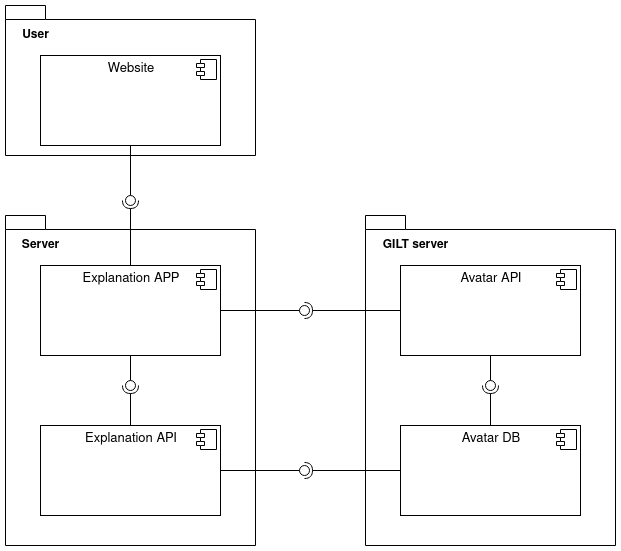
\includegraphics[scale=0.4]{component_diagram.png}
\caption{Component Diagram.} \label{fig1}
\end{figure}

A user interacts with the web application that was developed in React, an open-source JavaScript framework for building user interfaces.
Here the user can search of the desired concept as well as changing the page language.
This is also the place where the generated explanation are shown in plain text or in LGP by the avatar.
After each explanation, it is also presented their LGP Readability Score, which is presented more in depth in the following subsection, as well as feedback options.
If one of the presented explanations is not acceptable, it is possible for the user to request a new one.

When a concept is searched for, the input is sent to an API that was developed in Flask, a lightweight open-source Python web framework.
This API will generate a list of explanations using only web scrapping or a combination of web crawling, web scrapping and text summarization.
The approach to be used is set on its configuration file, and will depend on the initial source of information.
For websites where a single page can be a rich source of information like in Priberam\cite{priberam}, the first approach can yield good results.
On the hand, for websites where the information is scattered across many pages like Wikipedia\cite{wikipedia}, the second approach is ideal.

All the tasks that compose each approach were developed using Python libraries: Scrapy for web-crawling, Beautiful Soup for web scrapping and Natural Language Toolkit (NLTK) for text summarization.

The list of explanations is sorted based on each explanation LGP Readability Score, and the ones with the lowest score are selected.

The avatar and its database are projects that were previously developed by GILT and that are used to enhance this project.

\subsection{LGP Readability}

The developed API always generates more than one explanations and the number is even higher for words that have different meanings based on its context.
This explanations need to be sorted in order to present the user with the ones best suited for their needs.

For a regular language, there are metrics, like the readability score, that can be used to classify each expression in order to sort them accordingly.
This score indicates how easily a reader would comprehend the text that he's reading.

There are multiple formulas that could be used for calculating this score in Portuguese, as shown in table \ref{table:ptformulas}.
However there is none for the LGP.

When looking at the readability formulas for Portuguese, it is easy to notice that, all of them take in consideration the same variables, which are common in every written text: characters, complex words, syllables, words and sentences.

After analyzing the LGP signs, with the goal of creating a new readability calculation formula, all the shared variables where identified:

\begin{itemize}
    \item Hand configurations (CF) - The hand shape in a particular moment.
    \item Moments (MT) - The position of the hand in relation to the body.
    \item Hands (HS) - Both hands or only the dominant hand.
    \item Facial expressions (FE) - Motion or position of the face muscles.
\end{itemize}

Using those variables the following formula was created:

\begin{equation}
(0.7 \times CF + 0.3 \times MT + 1 \times FE) \times (0.5 \times HS)
\label{eqn1}
\end{equation}

The formula was tested using the signs from the avatar database and the constant values, that initially were set to 1, were manually adjusted to produce a more compact interval of results.
However, the constant value for the facial expressions was unaltered due to the current version of the avatar not supporting them.
In the table \ref{table:signs} is shown an example of some signs and its readability score.

\begin{table}[H]
    \centering
    \caption{Readability scores example.}
    \label{table:signs}
    \begin{tabular}{l|l|l|l|l}
        {\bfseries Sign} & {\bfseries CF} & {\bfseries MT} & {\bfseries HS} & {\bfseries Score} \\
        \hline
        Javali & 1 & 1 & 1 & 1.00  \\
        \hline
        Fornecedor & 2 & 6 & 1 & 2.09  \\
        \hline
        Auxílio & 2 & 4 & 2 & 3.59 \\
        \hline
        Consumo & 4 & 6 & 2 & 5.60 \\
        \hline
        Esclarecer & 7 & 7 & 2 & 8.00 \\
    \end{tabular}
\end{table}


\section{Contributions and Evaluation}

The main contribution is an application capable of helping in the learning process of a LGP user by allowing him to find explanations for a word or expression in his main language.
Another important contribution is a formula that can be used to calculate the readability of LGP content.
This can make it easier to produce said content, and by doing so, promoting the inclusion and equality of opportunities for the deaf community.

Although the project is not yet complete, the already developed functionality is capable of generate explanations in plain text using web crawling, web scrapping and text summarization and the avatar is able to translate plain text into LGP.
Thus is possible to corroborate the hypothesis that is possible to utilize Text Mining, Information Scraping and Information Retrieval techniques to generate the explanation of a given word or expression that does not exist in the LGP lexicon.

\section{Conclusions and Future Work}

In conclusion the project is still in development and this article presents a general view of it.

The LGP readability formula was able to produce a reliable scores when there was no need for signs that required facial expression.
However a new version of the avatar, that uses facial expressions, is being released which will allow to obtain values to calibrate the formula for the signs that do require facial expressions.

At the current stage, the application is able to produce explanations based on the word searched and show it to the user in plain text.
The explanation to be shown is not yet selected based on the readability formula.
In the cases where it was generated using only web scrapping, the selection was based on the order from the source page.
If it was generated using text summarization, the selection was based on the order created by its process.

Furthermore other functionality will still be implemented or changed to better fulfill the need of the target audience.
The main feature still to be implemented is the integration of the avatar that is responsible for translating the explanations displayed in plain text to LGP.
Another feature not yet implemented is the displaying of the LGP readability score next to each explanation.
Also the possibility for the user to ask for a new explanation if any of the ones available is deemed unacceptable.

In regards to future work, the project can target an even broader audience by supporting other languages which, the avatar, is capable of performing the translation from plain text to the corresponding sign language.
Additionally, the developed API may be used to further enhance the functionality of future or already existing GILT projects.


%
% ---- Bibliography ----
%
% BibTeX users should specify bibliography style 'splncs04'.
% References will then be sorted and formatted in the correct style.
%
% \bibliographystyle{splncs04}
% \bibliography{mybibliography}
%
\begin{thebibliography}{8}
    \bibitem{novak_2012}
        Novak, J.: Learning, creating, and using knowledge: concept maps as facilitative tools in schools and corporations. 2nd edn. Routlege, New York (2012)

    \bibitem{who_2020}
        WHO Deafness and hearing loss, \url{https://www.who.int/news-room/fact-sheets/detail/deafness-and-hearing-loss}. Last accessed 19 Aug 2020

    \bibitem{sts_2020}
        Spread The Sign Homepage, \url{https://www.spreadthesign.com/}. Last accessed 26 Aug 2020

    \bibitem{infopedia_2020}
        Infopédia Portuguese Sign Language dictionary, \url{https://www.infopedia.pt/dicionarios/lingua-gestual}. Last accessed 26 Aug 2020

    \bibitem{ctilg_2020}
        Ctilg Homepage, \url{http://www.ctilg.pt/}. Last accessed 27 Aug 2020

    \bibitem{serviin_2020}
        Serviin Homepage, \url{http://www.portaldocidadaosurdo.pt/Serviin}. Last accessed 27 Aug 2020

    \bibitem{ptread_2019}
        Antunes, H., Lopes, C.: Analyzing the adequacy of readability indicators to a non-english language.
        In: International Conference of the Cross-Language Evaluation Forum for European Languages,
        pages 149--155. Springer, 2019.

    \bibitem{priberam}
        Priberam Homepage \url{https://dicionario.priberam.org/}, Last accessed 5 Sep 2020

    \bibitem{wikipedia}
        Wikipedia Homepage \url{https://www.wikipedia.org/}, Last accessed 5 Sep 2020

        %\bibitem{ref_article1}
        %Author, F.: Article title. Journal \textbf{2}(5), 99--110 (2016)

        %\bibitem{ref_lncs1}
        %Author, F., Author, S.: Title of a proceedings paper. In: Editor,
        %F., Editor, S. (eds.) CONFERENCE 2016, LNCS, vol. 9999, pp. 1--13.
        %Springer, Heidelberg (2016). \doi{10.10007/1234567890}

        %\bibitem{ref_book1}
        %Author, F., Author, S., Author, T.: Book title. 2nd edn. Publisher,
        %Location (1999)

        %\bibitem{ref_proc1}
        %Author, A.-B.: Contribution title. In: 9th International Proceedings
        %on Proceedings, pp. 1--2. Publisher, Location (2010)

        %\bibitem{ref_url1}
        %LNCS Homepage, \url{http://www.springer.com/lncs}. Last accessed 4
        %Oct 2017
\end{thebibliography}
\end{document}
